\begin{center}
{\it{by Carlos Bautista, Leonardo de Lima, Ricardo D'Elia Matheus, Eduardo Pont\'on, Le\^onidas A. Fernandes do Prado, and Aurore Savoy-Navarro}}
\end{center}

\label{sec9:MCHMtthh}
%\medskip
%\noindent
%\textit{\bf Abstract:}
%We consider the production of one or two Higgs bosons in
%association with a top/anti-top pair in the context of Composite Higgs
%scenarios.  Our focus is on the minimal composite Higgs model, based
%on the symmetry breaking pattern $SO(5) \to SO(4)$.  In the top sector
%we consider two possibilities: fermion resonances in the fundamental
%$\bf 5$ representation of $SO(5)$ and in the symmetric ${\bf 14}$
%representation.  We simulate the ${t\bar t}h$ and ${\bar t}thh$
%processes in MadGraph, and present first results relevant for the
%14~TeV High Luminosity phase of the LHC, and the possible High Energy
%LHC upgrade at 27~TeV. Our main focus is on the non-resonant
%production of the previous final states.
%%%%%%%%%%%%%%%%%%%%%%%%%%%%%%%%%%%%%
%\subsubsection{Introduction}
%%%%%%%%%%%%%%%%%%%%%%%%%%%%%%%%%%%%%
With the discovery of the Higgs boson~\cite{Aad:2012tfa,
CMSHiggsJuly2012} the question of whether this resonance is a
composite state has gained new prominence.  We consider the effects of
Higgs compositeness~\cite{Kaplan:1983fs, Kaplan:1983sm, Georgi:1984ef, Georgi:1984af, Dugan:1984hq} on the $t\bar{t}h$ and
$t\bar{t}  h h$ processes.  The first process has already been
observed~\cite{Aaboud:2018urx, Sirunyan:2018hoz}, and is consistent
with the SM expectation, although with large uncertainties of order
20\%.  The second process is of particular interest, due to the contribution of charge 2/3 vector-like ``top partners" decaying in the $tH$ channel. Searches focusing on
this channel have been presented in~\cite{Aaboud:2018xuw}, and
combined ones that consider the $bW$, $tZ$ and $tH$ channels
already put strong constraints on such vector-like
resonances~\cite{Aaboud:2018pii, Sirunyan:2018omb}.
%With the discovery of the Higgs boson~\cite{Aad:2012tfa,
%CMSHiggsJuly2012} the question of whether this resonance is a
%composite state, or rather the first observed scalar particle %that
%appears elementary down to distances much shorter than its %Compton
%wavelength, has gained new prominence.  We consider the question %of
%Higgs compositeness~\cite{Kaplan:1983fs, Kaplan:1983sm, %Georgi:1984ef, Georgi:1984af, Dugan:1984hq} and the possible %effects on the $t\bar{t}h$ and
%$t\bar{t}  h h$ processes.  The first one has already been
%observed~\cite{Aaboud:2018urx, Sirunyan:2018hoz}, and is %consistent
%with the SM expectation, although with large uncertainties of %order
%20\%.  The second one is of particular interest for the models we
%consider, since one expects new charge 2/3 vectorlike ``top %partners"
%that can decay in the $th$ channel.  Resonance searches focusing %on
%this decay channel have been presented in~\cite{Aaboud:2018xuw}, %and
%combined searches that consider the $bW$, $tZ$ and $th$ channels
%already put strong constraints on such vectorlike
%resonances~\cite{Aaboud:2018pii, Sirunyan:2018omb}.

In this work, we point out the non-resonant ${t\bar t}hh$ process is of considerable interest, since in light of these strong bounds it will very often account for a large fraction of the total ${t\bar t}hh$ cross-section. Furthermore, it carries
information about the compositeness nature of the Higgs boson that is distinct and complimentary to the effect of the heavy fermion resonances. We also point out that the non-resonant
${t\bar t}hh$ process is closely connected to ${\bar t}th$, but would be expected to display larger deviations from the
SM prediction.  We present here a first step in the analysis of such
processes in the context of the HL-LHC and HE-LHC for the ``Minimal Composite Higgs
Models" (MCHM)~\cite{Agashe:2004rs}, in which the Higgs doublet is identified with the pseudo-Nambu-Goldstone bosons originating from the breaking $SO(5) \to SO(4)$ by new strong dynamics, with $SO(4)$ weakly gauged by the SM gauge group. We refer the
reader to the full review in~\cite{Panico:2015jxa} for complete
details on Composite Higgs.  Further details on our work
 can be found in the companion paper~\cite{MCHMtthh}.

%In this work, we point out that the non-resonant ${t\bar t}hh$ process
%is also of considerable interest in this context.  Due to the already
%existing strong bounds on the vectorlike resonances, the non-resonant
%production very often accounts for a large fraction of the total
%${t\bar t}hh$ cross-section.  Furthermore, it carries distinct
%information about the compositeness nature of the Higgs boson, as
%opposed to the indirect information connected to the existence of the
%heavy fermion resonances.  We also point out that the non-resonant
%${t\bar t}hh$ process is closely connected to the ${\bar t}th$
%process, but would be expected to display larger deviations from the
%SM prediction.  We present here a first step in the analysis of such
%processes in the context of the 14~TeV High Luminosity phase of the
%LHC, and the possible High Energy LHC upgrade at 27~TeV. We explore
%these questions in the framework of the ``Minimal Composite Higgs
%Models"~\cite{Agashe:2004rs}, considering two possible
%realizations of the sector of fermionic resonances.  Further details
%can be found in the companion paper~\cite{MCHMtthh}.

%%%%%%%%%%%%%%%%%%%%%%%%%%%%%%%%%%%%%
\subsubsection*{Theoretical Framework}
\label{MCHM}
%%%%%%%%%%%%%%%%%%%%%%%%%%%%%%%%%%%%%
In composite Higgs models, physical states are linear superpositions of the strong sector composite resonances
and the SM-like ``elementary" states with the same quantum numbers, realising the paradigm of partial
compositeness ~\cite{KAPLAN1991259}.
%The modern composite Higgs paradigm posits a new strongly coupled
%sector that spontaneously breaks a global symmetry ${\cal G}$ %down to
%a subgroup ${\cal H}$, thus generating a number of
%pseudo-Nambu-Goldstone bosons, some of which are identified
%with the Higgs doublet.  The SM gauge group is contained in ${\cal H}$
%and electroweak symmetry breaking takes place only when the 5Higgs
%doublet acquires a vacuum expectation value, a process that is
%dynamical and often calculable in such scenarios.  In addition to a
%set of strong resonances of various spins, there is an ``elementary"
%sector that mimics in its gauge quantum numbers the Standard Model.  The physical states are linear superpositions of the composite
%and elementary states, realizing the paradigm of partial
%compositeness, first proposed in~\cite{KAPLAN1991259}.  We refer the
%reader to the full review in~\cite{Panico:2015jxa} for complete
%details.  We restrict ourselves here to the MCHM scenarios, where
%${\cal G} = SO(5)$ and ${\cal H} = SO(4)$.
We focus on the top sector,
which is the most relevant to the processes we study. (See Section~\ref{sect-illus} for a complementary study on Higgs coupling to gauge bosons).  Here we present only the essential features of the
 analysis, referring the reader to the companion
work~\cite{MCHMtthh} for further details. Two concrete
realisations of the fermionic sector are adopted. Both share an elementary sector denoted by $q_L$ and
$t_R$, transforming  as $(3,2,1/6)$ and $(3,1,2/3)$ under the SM gauge group.
%In this work, we focus on the resonances associated to the top sector,
%as these are the most relevant to the processes we study. Note Section~\ref{sect-illus} for a complementary study on Higgs coupling to gauge bosons.  We
%summarize here the essential features that enter into the
%phenomenological analysis, referring the reader to the companion
%work~\cite{MCHMtthh} for precise conventions and further details.
%Since the fermionic sector is model dependent, we adopt two concrete
%realizations.  Both share an elementary sector denoted by $q_L$ and
%$t_R$, described by
%
%\bea
%\mathcal{L}_{\rm elem} &= \bar{q}_L i \slashed{D} q_L +\bar{t}_R %i \slashed{D} t_R~,
%\label{elem}
%\eea
%%
%where $D$ stands for the $SU(3)_C \times SU(2)_L \times U(1)_Y$
%covariant derivative.  $q_L$ and $t_R$ transform as $(3,2,1/6)$ and
%$(3,1,2/3)$ under the SM gauge group.

\medskip
\noindent
\textit{\small \bf The MCHM$_5$}
\medskip

In this ``minimal" extension, one considers fermion resonances in a 
${\bf 5}$ of $SO(5)$, which splits into a $SO(4)$ 4-plet,
$\Psi_4$, with mass $M_4$, and a $SO(4)$ singlet, $\Psi_1$, with mass $M_1$.
%In this ``minimal" extension, one considers fermion resonances in a 
%${\bf 5}$ of $SO(5)$, which splits into a $SO(4)$ 4-plet,
%$\Psi_4$, and a $SO(4)$ singlet, $\Psi_1$:
%
\be
\Psi_4 ~\sim~ (X_{5/3}, X_{2/3}, T, B)~;~   \Psi_1 ~\sim~ \tilde{T}~.
\label{comp5content}
\ee
%

 The states $(X_{5/3}, X_{2/3})$ transform as a $SU(2)_L$ doublet with $Y = 7/6$, while $(T, B)$ and $\tilde{T}$ transform like $q_L$ and $t_R$, respectively. These are not mass eigen-states due to the mixing with elementary states, described here by ~\footnote{In principle, one can
choose different Yukawa couplings for the terms involving the ${\bf 4}$-plet, $\Psi_4$, and the singlet, $\Psi_1$.
See~\cite{MCHMtthh}.}
 %The states $(X_{5/3}, X_{2/3})$ transform as a $SU(2)_L$ doublet with
 %exotic hypercharge $Y = 7/6$.  The states $(T, B)$ also transform as
 %a $SU(2)_L$ doublet and have hypercharge $Y = 1/6$, while $\tilde{T}$
 %is a $SU(2)_L$ singlet with hypercharge $Y = 2/3$.  The composite
 %sector is described by
%
%\bea
%\mathcal{L}^{\mathbf{5}}_{\rm comp} &=&
% \bar{\Psi}_{\mathbf{4}} i \slashed{D} \Psi_{\mathbf{4}}-M_4 %\bar{\Psi}_{\mathbf{4}} \Psi_{\mathbf{4}}+ %\bar{\Psi}_{\mathbf{1}} i \slashed{D} \Psi_{\mathbf{1}}-M_1 %\bar{\Psi}_{\mathbf{1}} \Psi_{\mathbf{1}}~.
%\label{comp5}
%\eea
%
%There is also the possibility of mixing between the composite and
%elementary states, described here by~\footnote{In principle, one can
%choose different Yukawa couplings for the terms involving the %${\bf 4}$-plet, $\Psi_4$, and the singlet, $\Psi_1$.
%See~\cite{MCHMtthh}.}
%
\bea
\mathcal{L}^{\mathbf{5}}_{\rm mix} &=&
y_L f \, \bar{q}_L^{\mathbf{5}} U \left[ \Psi_{\mathbf{4}} + \Psi_{\mathbf{1}} \right] 
+ y_R f \, \bar{t}_R^{\mathbf{5}} U \left[ \Psi_{\mathbf{4}} + \Psi_{\mathbf{1}} \right] + \mathrm{h.c.}
\label{Lmix5}
\eea
%
where $U$ parametrises the Higgs field and $f$ is the ``Higgs decay
constant".  All the features required for our analysis follow from diagonalisation of the charge 2/3 fermion mass matrix, which is given in Ref.~\cite{MCHMtthh}, while the
 remaining resonances have masses $M_{X_{5/3}} = M_4$ and $M_B =
\sqrt{M_4^2 + y_{L}^2 f^2}$. Deviations from a SM Higgs due to compositeness are characterised by the parameter $\xi = v^2/f^2$ (here $v = 246~{\rm \UGeV}$). Consistency with current
Higgs measurements results in $\xi\lesssim 0.1$, or $f \gtrsim 800$
\UGeV~\cite{Falkowski:2013dza, Carena:2014ria, Buchalla:2014eca,
Sanz:2017tco, Liu:2017dsz, Banerjee:2017wmg, deBlas:2018tjm}.  

%All the features required for our analysis follow from the charge 2/3 fermion mass matrix, given in the $\{{\bar t}_L,~{\bar
%T}_L,~{\bar X}_{2/3, L},~\overline{\tilde{T}}_L\}$ vs
%$\{t_R,~T_R,~X_{2/3, R},~\tilde{T}_R\}$ basis by
%
%\begin{align}
%\mathcal{M}_{2/3}^{\mathbf{5}} =
%\left[\begin{array}{cccc}
%        0 & \frac{1}{2} y_{L} f (1+\sqrt{1-\xi}) & \frac{1}{2} y_{L} f (1-\sqrt{1-\xi}) & \frac{1}{\sqrt{2}} y_{L} f \sqrt{\xi} \\
%        -\frac{1}{\sqrt{2}} y_{R} f \sqrt{\xi} & -M_4 & 0 & 0 \\
%        \frac{1}{\sqrt{2}} y_{R} f \sqrt{\xi} & 0 & -M_4 & 0 \\
%        y_{R} f \sqrt{1-\xi} & 0 & 0 & -M_1
%      \end{array}\right]~,
%\label{e:mass5}
%\end{align}
%
%where $\xi = v^2/f^2$ characterizes the deviations from a SM Higgs due
%to compositeness (here $v = 246~{\rm GeV}$).
%Consistency with current
%Higgs measurements results in $\xi\lesssim 0.1$, or $f \gtrsim %800$
%GeV~\cite{Falkowski:2013dza, Carena:2014ria, Buchalla:2014eca,
%Sanz:2017tco, Liu:2017dsz, Banerjee:2017wmg, deBlas:2018tjm}.  The
%remaining resonances have masses $M_{X_{5/3}} = M_4$ and $M_B =
%\sqrt{M_4^2 + y_{L}^2 f^2}$.

\medskip
\noindent
\textit{\small \bf The MCHM$_{14}$}
\medskip

In the second scenario, the composite states span a ${\bf 14}$ of
$SO(5)$~\cite{Pomarol:2012qf, Panico:2012uw, Montull:2013mla, 
Carena:2014ria, Carmona:2014iwa, Kanemura:2016tan, Gavela:2016vte, 
Liu:2017dsz}. Under $SO(4)$, in addition to a 4-plet and a singlet, as in
Eq.~(\ref{comp5content}), we have an additional $SO(4)$ nonet:
%
\bea
\Psi_{\bf 9} &\sim& (U_{8/3}, U_{5/3}, U_{2/3}, Y_{5/3}, Y_{2/3}, Y_{-1/3}, Z_{2/3}, Z_{-1/3}, Z_{-4/3})~.
\eea
%
The $U$'s, $Y$'s and $Z$'s transform as $SU(2)_L$ triplets, with
hyper-charges $Y = 5/3$, $2/3$ and $-1/3$, respectively. The 
Lagrangian of the MCHM$_5$ is supplemented by terms
involving $\Psi_9$, whose mass is denoted $M_9$, and which mixes with the elementary states in an analogous manner to $\Psi_1$ and $\Psi_4$.
%The $U$'s, $Y$'s and $Z$'s transform as $SU(2)_L$ triplets, with
%hypercharges $Y = 5/3$, $2/3$ and $-1/3$, respectively.  The composite
%Lagrangian given in Eq.~(\ref{comp5}) is supplemented by terms
%involving $\Psi_9$:
%
%\bea
%\mathcal{L}^{\mathbf{14}}_{\rm comp} &=& %\mathcal{L}^{\mathbf{5}}_{\rm comp} +
%\mathrm{Tr}\left[\bar{\Psi}_{\mathbf{9}} i %\slashed{D}\Psi_{\mathbf{9}} \right]-M_9 %\mathrm{Tr}\left[\bar{\Psi}_{\mathbf{9}} %\Psi_{\mathbf{9}}\right]~,
%\eea
%
%while the mixing with the elementary states is given by~\footnote{Here
%$Q_L^{\bf 14}$ and $T_R^{\bf 14}$ are convenient extensions of $q_L$
%and $t_R$ that simplify the writing of the Lagrangian.
%See~\cite{MCHMtthh}.}
%
%\bea
%\mathcal{L}^{\mathbf{14}}_{\rm mix} &=&
%y_L f \, {\rm Tr} \left[ U^\mathsf{T} \bar{Q}_L^{\mathbf{14}} U \Psi_{\mathbf{14}} \right]
%+ y_R f \, {\rm Tr} \left[ U^\mathsf{T} \bar{T}_R^{\mathbf{14}} U
%\Psi_{\mathbf{14}} \right] + \mathrm{h.c.}
%\label{Lmix14}
%\eea
%
%where $\Psi_{\bf 14} \equiv \Psi_{\mathbf{9}} + \Psi_{\mathbf{4}} + \Psi_{\mathbf{1}}$.
We give the full charge $2/3$ and $-1/3$ mass matrices as well as the complete Lagrangian in Ref.~\cite{MCHMtthh}. The remaining states have masses
$M_{X_{5/3}} = M_4$, $M_{U_{8/3}} = M_{U_{5/3}} = M_{Y_{5/3}} =
M_{Z_{-4/3}} = M_9$.

%The charge 2/3 mass matrix, in the $\{{\bar t}_L,~{\bar %T}_L,~{\bar
%X}_{2/3, L},~\overline{\tilde{T}}_L,~{\bar U}_{2/3, L},~{\bar %Y}_{2/3,
%L},~{\bar Z}_{2/3, L}\}$ vs 
%$\{t_R,~T_R,$ $X_{2/3, R},~\tilde{T}_R,~U_{2/3, R},~Y_{2/3, %R},~Z_{2/3, R}\}$ basis, is given by:
%
%{ \small
%\begin{align}
%&\mathcal{M}_{2/3}^{\mathbf{14}} =
%&\left[\begin{array}{ccccccc}
%        0 & \frac{1}{2} y_{L} f a_+ & -\frac{1}{2} y_{L} f a_- & -\frac{\sqrt{5}}{4} y_{L} f s_{2h} & -\frac{1}{2} y_{L} f b_- &-\frac{1}{2} y_{L} f s_{2h} &\frac{1}{4} y_{L}f b_+ \\
%        \frac{\sqrt{5}}{4} y_{R} f s_{2h} & -M_4 & 0 & 0&0&0& 0\\
%        -\frac{\sqrt{5}}{4} y_{R} f s_{2h} &0& -M_4  & 0&0&0& 0\\
%        y_{R}f\left(1-\frac{5}{4} s^2_h \right) & 0 & 0 & -M_1&0&0&0 \\
%        \frac{\sqrt{5}}{4} y_{R} f s^2_h & 0 & 0 &0 & -M_9&0&0 \\
%        -\frac{\sqrt{5}}{4} y_{R} f s^2_h &0 &0 &0 &0&-M_9&0 \\
%        \frac{\sqrt{5}}{4} y_{R} f s^2_h & 0 & 0 &0 & 0&0&-M_9
%      \end{array}\right]~,
%\label{e:mass14}
%\end{align}
%}
%
%where
%$
%s^2_{h} = \xi~,
%\hspace{1em}
%s_{2h} = 2\sqrt{\xi}\sqrt{1-\xi}~,
%\hspace{1em}
%a_\pm = 1 \pm \sqrt{1-\xi} - 2\xi~,
%\hspace{1em}
%b_\pm = \sqrt{\xi} \left(1 \pm \sqrt{1-\xi} \right)
%$.

%We give the charge $-1/3$ mass matrix in Ref.~\cite{MCHMtthh}, as it
%plays a subdominant role. The remaining states have masses
%$M_{X_{5/3}} = M_4$, $M_{U_{8/3}} = M_{U_{5/3}} = M_{Y_{5/3}} =
%M_{Z_{-4/3}} = M_9$. 


An important distinction between the two scenarios is that when the
mixing is dominated by the nonet, the leading order operator coupling
the top quark to the Higgs doublet is the non-renormalisable operator
${\bar q}_L \tilde{H} t_R H^\dagger H$.  In contrast, mixing through a
4-plet or singlet lead to the SM operator ${\bar q}_L \tilde{H} t_R$
(plus corrections that are higher order in $v/f$).  In the former case
the ratio of the top Yukawa coupling to the top mass is three times
larger than in the second case.  Cases where the nonet plays a
comparable role to the 4-plet or singlet can then lead to interesting
enhancements in the top Yukawa coupling, which are not present in the
MCHM$_5$.

The scenarios under consideration can also affect the Higgs decays. Once the light fermion representations are chosen, and assuming their mixing angles are small, one can express the partial widths as
a rescaling of the corresponding SM widths. For further details, we refer to ~\cite{MCHMtthh}.
%\medskip
%\noindent
%\textit{\small \bf Higgs Decays}
%\medskip

%The scenarios under consideration can also affect the Higgs decays,
%and thus require a specification of how the remaining (light) fermions
%are treated.  For concreteness, we assume that the RH bottom is
%associated with resonances in a ${\bf 10}$ of
%$SO(5)$~\cite{Carena:2014ria}.  For the remaining fermions, we %choose
%to replicate the scheme employed for the third family.  We also assume
%that the lepton sector follows the same scheme as the quark sector.
%Furthermore, we assume that the mixing angles between the elementary
%and composite states associated with the light families are small, as
%in ``anarchy" models of flavor.

%Under the previous assumptions, one can express the partial widths as
%a rescaling of the corresponding SM widths.  For the MCHM$_5$, %one
%finds~\cite{Carena:2014ria}
%
%\bea
%\Gamma(h \to b {\bar b}) &=& F_2(\xi)^2 \, \Gamma_{\rm SM}(h \to %b {\bar b})~,
%\nonumber \\ [0.5em]
%\Gamma(h \to c {\bar c}) &=& F_1(\xi)^2 \, \Gamma_{\rm SM}(h \to %c {\bar c})~,
%nonumber \\ [0.5em]
%\Gamma(h \to \tau^+ \tau^-) &=& F_2(\xi)^2 \, \Gamma_{\rm SM}(h %\to \tau^+ \tau^-)~,
%\\ [0.5em]
%\Gamma(h \to VV) &=& F_2(\xi)^2 \, \Gamma_{\rm SM}(h \to VV)~,
%\nonumber \\ [0.5em]
%\Gamma(h \to gg) &=& F_1(\xi)^2 \, \Gamma_{\rm SM}(h \to gg)~,
%\nonumber
%\eea
%where
%\be
%F_1(\xi) ~=~ \frac{1-2\xi}{\sqrt{1-\xi}}~,
%\hspace{1cm}
%F_2(\xi) ~=~ \sqrt{1-\xi}~.
%\label{Ffunctions}
%\ee
%

%For the MCHM$_{14}$, the bottom channel is controlled by $F_1$ %instead
%of $F_2$, and the $ggh$ coupling is controlled by
%
%\bea
%c_g^{\bf 14} &\approx&
%\frac{
%4 \left(1 - r_1\right) r_9
%- \left(9 r_1 + 23 r_9 - 32 r_1 r_9\right) \xi
%+ 4 \left(3 r_1 + 5 r_9 - 8 r_1 r_9\right) \xi ^2
%}
%{\sqrt{1-\xi }
%\left[4 \left(1 - r_1 \right) r_9 - \left(3 r_1 + 5 r_9 - 8 r_1 %r_9\right) \xi \right]}~,
%\eea
%
%where $r_1 = M_1 / M_4$ and $r_9 = M_9 / M_4$, instead of %$F_1(\xi)$.

%The total Higgs width in the MCHM models under consideration can %then
%be written as
%
%\bea
%\Gamma_5(h) &=& \left\{ F_2(\xi)^2 \left[ {\rm BR_{\rm SM}(b{\bar %b})} + {\rm BR_{\rm SM}(VV)} + {\rm BR_{\rm SM}(\tau^+ \tau^-)} %\right] \right.
%\nonumber \\
%&& \mbox{} + \left. F_1(\xi)^2 \left[ {\rm BR_{\rm SM}(gg)} + {\rm BR_{\rm SM}(c{\bar c})} \right] \right\} \Gamma_{\rm %SM}(h)~,
%\\ [0.5em]
%\Gamma_{14}(h) &=& \left\{ F_2(\xi)^2 \left[{\rm BR_{\rm SM}(VV)} %+ {\rm BR_{\rm SM}(\tau^+ \tau^-)} \right] \right.
%\nonumber \\
%&& \mbox{} + \left. F_1(\xi)^2 \left[ {\rm BR_{\rm SM}(b{\bar %b})} + {\rm BR_{\rm SM}(c{\bar c})} \right]
%+ (c_g^{\bf 14})^2 \, {\rm BR_{\rm SM}(gg)} \right\} \Gamma_{\rm %SM}(h)~,
%\eea
%
%and the branching fractions can also be written in terms of the
%functions $F_1$, $F_2$, $c_g^{\bf 14}$, and SM quantities.  They
%These branching fractions 
%are all that is needed to take into account the
%effects of compositeness in Higgs decays.
%%%%%%%%%%%%%%%%%%%%%%%%%%%%%%%%%%%%%%%%%%%%%%%%
\subsubsection*{Parameter Space and Results}
\label{analysis}
%%%%%%%%%%%%%%%%%%%%%%%%%%%%%%%%%%%%%%%%%%%%%%%%
Taking all parameters to be real for simplicity, the free parameters can be taken to be $f$, $|M_1|$, $|M_4|$, ${\rm sign}(M_1)$, $y_L$ and $y_R$, common for both models, plus $|M_9|$ and ${\rm sign}(M_4)$ for the MCHM$_{14}$.
%The parameters of the models are $M_i$, $f$, $y_L$ and $y_R$. For simplicity, we
%will take all parameters to be real, so that the free parameters can be
%taken as follows:
%\begin{itemize}
%\item MCHM$_5$: $f$, $|M_1|$, $|M_4|$, ${\rm sign}(M_1)$, $y_L$ and $y_R$.
%\item MCHM$_{14}$: $f$, $|M_1|$, $|M_4|$, $|M_9|$, ${\rm sign}(M_1)$, ${\rm sign}(M_4)$, $y_L$ and $y_R$.
%\end{itemize}
Out of these, we choose to fix $y_R$ to reproduce the top mass. Running of this mass from the scale of the resonances, typically around $2-3$ \UTeV to the relevant scales for $t\bar{t}hh$ of the order of a
couple hundred \UGeV is taken into account to a first approximation by using a running top mass of $\bar{m}_t = 150$ \UGeV for the diagonalisation of the mass
matrix, and of $m_t = 173$ \UGeV, for the kinematic quantities.   We take the Higgs mass as an independent parameter,
referring the reader to~\cite{MCHMtthh} for further discussion on this point.
%One of these parameters can be further fixed by requiring that the top
%mass be reproduced.  We choose to fix $y_R$ in this way.  We use here
%the running top mass at the scale of the resonances, which will be
%typically around $2-3$~TeV. We take $\bar{m}_t = 150$~GeV. For
%$t\bar{t}h$, and also for the parts of $t\bar{t}hh$ to be %described in
%the following Section, the relevant scales are of the order of a
%couple hundred GeV. We therefore distinguish between the high-scale
%running top mass (relevant for the diagonalization of the mass
%matrix), and a low scale running top mass, relevant to the physical
%processes of interest.  We take for the latter the pole top mass of
%$m_t = 173$~GeV, which also enters in kinematical quantities.  To
%first approximation, this takes into account the running between the
%two scales.  We take the Higgs mass as an independent parameter,
%referring the reader to~\cite{MCHMtthh} for further discussion on this
%point.

We consider the following ranges for the parameters (those common to both models take the same range):
\begin{align*}
|M_1|& \in [800, 3000]~{\rm \UGeV}~, &  |M_4| &\in [1200, 3000]~{\rm \UGeV}~,  &  M_9 &\in [1300, 4000]~{\rm \UGeV}~,  \\
f&\in [800, 2000]~{\rm \UGeV}~,          &  y_L&\in [0.5, 3] ~.
\end{align*}
%For the MCHM$_5$, we consider the following ranges for the parameters:
%\begin{align*}
%|M_1|& \in [800, 3000]~{\rm GeV}~, &  M_4 &\in [1200, 3000]~{\rm GeV}~,  \\
%f&\in [800, 2000]~{\rm GeV}~,          &  y_L&\in [0.5, 3] ~.
%\end{align*}
%
%For the MCHM$_{14}$, we use:
%\begin{align*}
%|M_1|& \in [800, 3000]~{\rm GeV}~, &  |M_4| &\in [1200, %3000]~{\rm GeV}~,  &  M_9 &\in [1300, 4000]~{\rm GeV}~,  \\
%f&\in [800, 2000]~{\rm GeV}~,          &  y_L&\in [0.5, 3] ~.
%\end{align*}
We take $y_L < 3$ and check that $y_R < 4$, in order to remain in the (semi-) perturbative regime.
%We take an upper limit on $y_L < 3$, in order to remain in the %(semi-)
%perturbative regime and thus justify the present tree-level analysis.
%For the same reason, we also check that $y_R$, as determined by %the
%top mass, is below 4.
%
\begin{figure}[t]
\centering
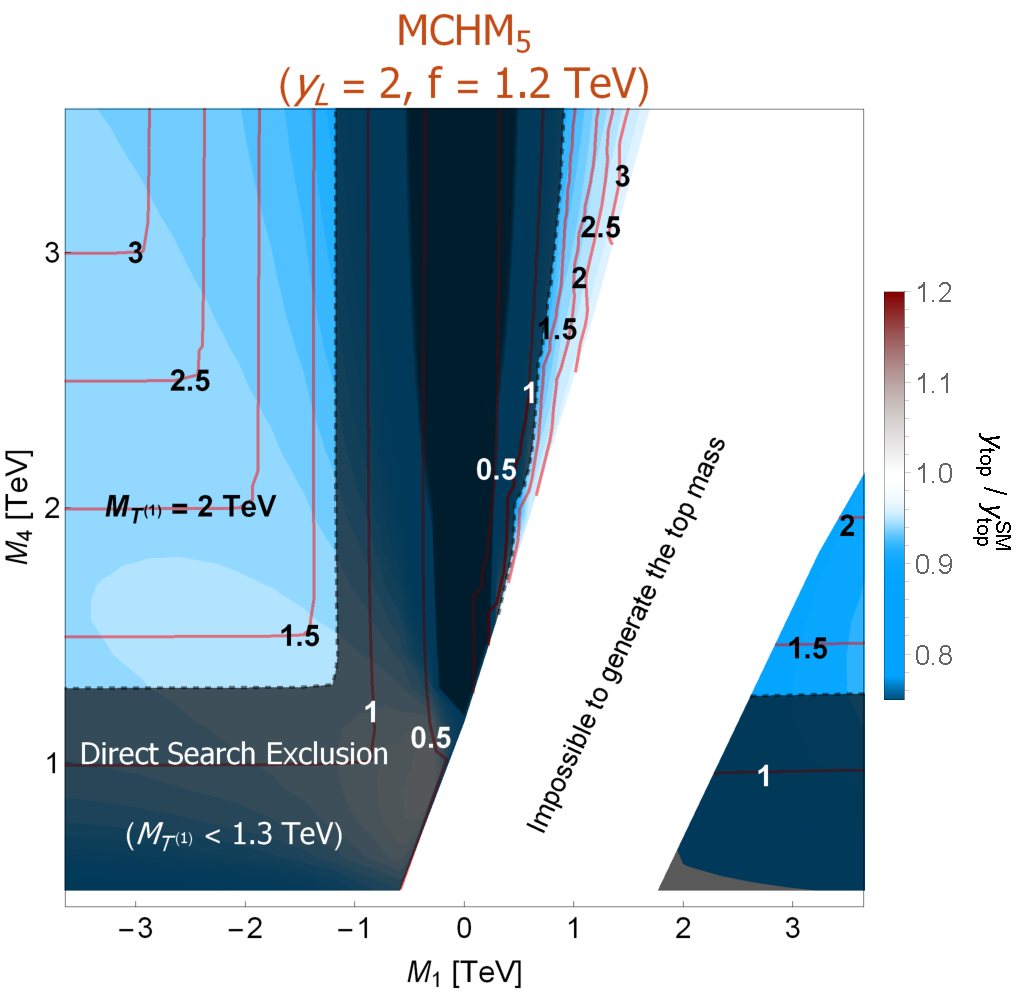
\includegraphics[width=0.475\textwidth]{\main/section9/plots/MCHM5_gridplot.pdf}
\hspace{3mm}
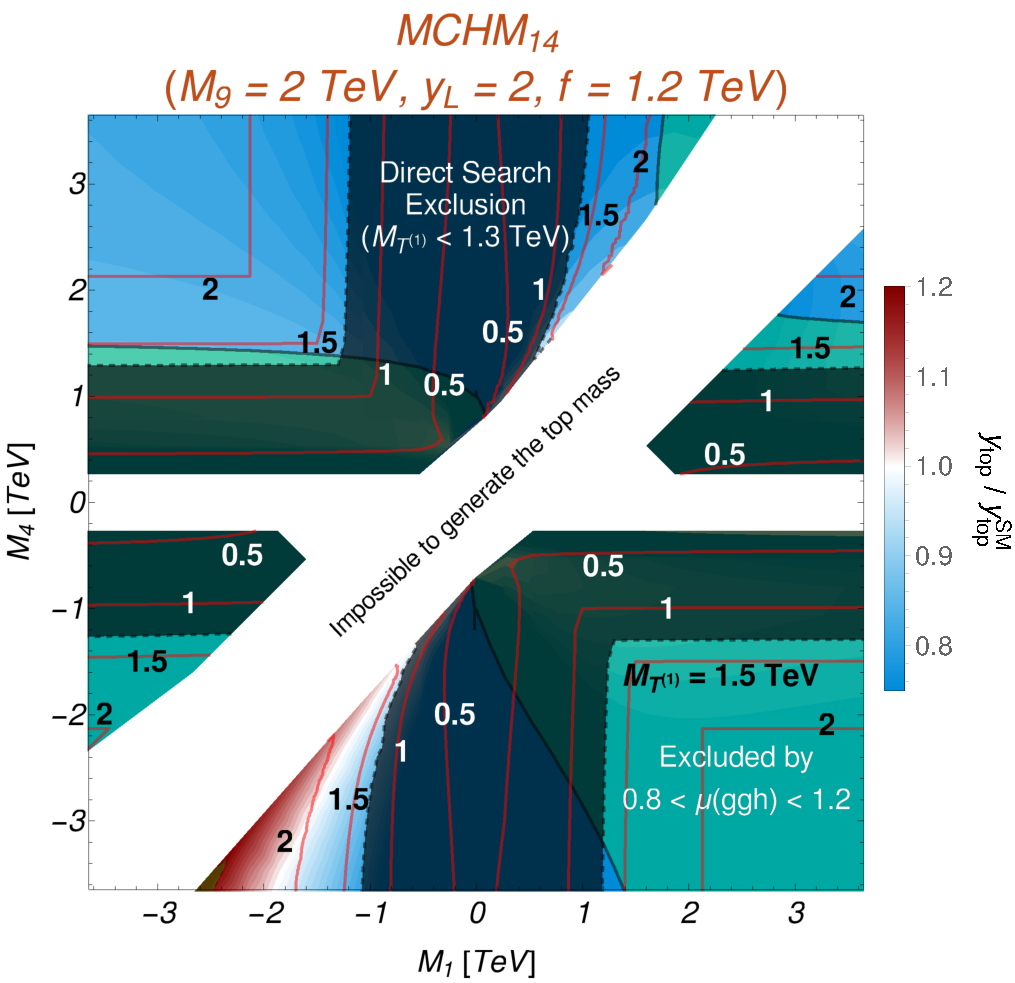
\includegraphics[width=0.485\textwidth]{\main/section9/plots/MCHM14_GridPlot_f_1200_M9_2TeV.pdf}
\caption{Display of the values of the normalised top Yukawa coupling,
$y_{\rm top} / y_{\rm top}^{\rm SM}$, in the $M_1$-$M_4$ plane.  Blue
colours indicate a suppression and red colours an enhancement.  Also
shown the curves of constant $M_{T^{(1)}}$, the mass of the lightest $Q=2/3$
vector-like resonance.  The darker bands indicate the approximate
current direct exclusion of top partner VLQ resonances, assuming decays into
$bW$, $tZ$ and $tH$ ~\cite{Aaboud:2018pii, Sirunyan:2018omb}.}
\label{fig:ytvsM1M4}
\end{figure}
%
In Fig.~\ref{fig:ytvsM1M4} we show the normalised top Yukawa coupling,
$y_{\rm top} / y_{\rm top}^{\rm SM}$, in the $M_1$-$M_4$ plane for
both the MCHM$_5$ and MCHM$_{14}$ scenarios.  We fix $y_L = 2$ and $f
= 1200$~\UGeV, and $M_9 = 2$~\UTeV for the MCHM$_{14}$.  In the MCHM$_5$,
the scaling with $f$ is, to first approximation, given by the function
$(1-2\xi)/\sqrt{1-\xi}$, while for the MCHM$_{14}$ it is
intertwined with the other parameters in a more complicated way.  We
see that the MCHM$_5$ always displays a suppression of the top Yukawa
coupling compared to the SM limit, while the MCHM$_{14}$ can display
an enhancement in certain regions of parameter space, as pointed out
in~\cite{Liu:2017dsz}.  We also show in the figure, curves of constant
$M_{T^{(1)}}$ (red lines) and the approximate direct exclusion region
(dark bands).  The white area corresponds to the region in parameter
space where it is not possible to reproduce the top quark mass.  We
also show the region where the $ggh$ coupling deviates by more than
20\% from unity, as this region is expected to be in tension with the
current constraints on Higgs couplings~\cite{Khachatryan:2016vau}.
%%%%%%%%%%%%%%%%%%%%%%%%%%%%%%%%%%%%%%%%%%%%%%%%
%\subsubsubsection{Implementation into Event Generator}
%\label{mg}
%%%%%%%%%%%%%%%%%%%%%%%%%%%%%%%%%%%%%%%%%%%%%%%%
%We implement both models in FeynRules
%(v2.3)~\cite{Alloul:2013bka} and produce an associated UFO file for
%each model, that can be interfaced with MadGraph 5
%(v2.6.2)~\cite{Alwall:2014hca}.  The numerical input from the
%diagonalization of the mass matrices is then fed via a custom-written
%Python script into the param\_card.dat for processing within MG5.  We
%simulate the ${t\bar t} h$ and ${t\bar t} hh$ processes in MG5.  The 
%output is then ready to be run through PYTHIA~8.2~\cite{Sjostrand:2014zea}, which
%takes care of the decays of the top quarks and the Higgs.  We code the
%Higgs branching fractions, as described above,
%into Pythia.  We also check that the deviations from the SM in
%the top quark properties are negligible, since the new physics is
%rather heavy.  The output is then ready to pass through fast 
%simulation~\cite{deFavereau:2013fsa} or the full simulation of the LHC experiments for HL-LHC.

%%%%%%%%%%%%%%%%%%%%%%%%%%%%%%%%%%%%%%%%%%%%%%%%
\subsubsubsection*{The $t\bar{t}h$ Process}
\label{tth}
%%%%%%%%%%%%%%%%%%%%%%%%%%%%%%%%%%%%%%%%%%%%%%%%
To an excellent approximation, the $t\bar{t} h$ process in the MCHM
is related to the corresponding SM process by a simple rescaling of $\sigma_{\rm MCHM}(t\bar{t}h) ~=~ \left( y_t/y_t^{\rm SM} \right)^2 \, \sigma_{\rm SM}(t\bar{t}h)~.
\label{sigmatth}$
All the modifications due to Higgs compositeness, or mixing with
vector-like fermions, enter only through the top Yukawa coupling.
Therefore, only a modification in the total rate is expected, but not in kinematic distributions.
%To an excellent approximation, the $t\bar{t} h$ process in the MCHM
%is related to the corresponding SM process by a simple rescaling:
%
%\be
%\sigma_{\rm MCHM}(t\bar{t}h) ~=~ \left( \frac{y_t}{y_t^{\rm SM}} %\right)^2 \, \sigma_{\rm SM}(t\bar{t}h)~.
%\label{sigmatth}
%\ee
%
%All the modifications due to Higgs compositeness, or mixing with
%vector-like fermions, enter only through the top Yukawa coupling.
%Therefore, only a modification in the total rate is expected, but not in kinematic distributions.

%%%%%%%%%%%%%%%%%%%%%%%%%%%%%%%%%%%%%%%%%%%%%%%%
\subsubsubsection*{The $t\bar{t}hh$ Process}
\label{tthh}
%%%%%%%%%%%%%%%%%%%%%%%%%%%%%%%%%%%%%%%%%%%%%%%%
For the $t\bar{t}hh$ process there are two qualitatively different
contributions:
%
\begin{enumerate}
\item Resonant processes, involving the production and decay (in the
$th$ channel) of heavy vector-like states of charge 2/3 (top partners).
\item Non-resonant processes: these are defined by the diagrams that
do not involve the production of the vector-like resonances.
\end{enumerate}
%
\begin{figure}[t]
\centering
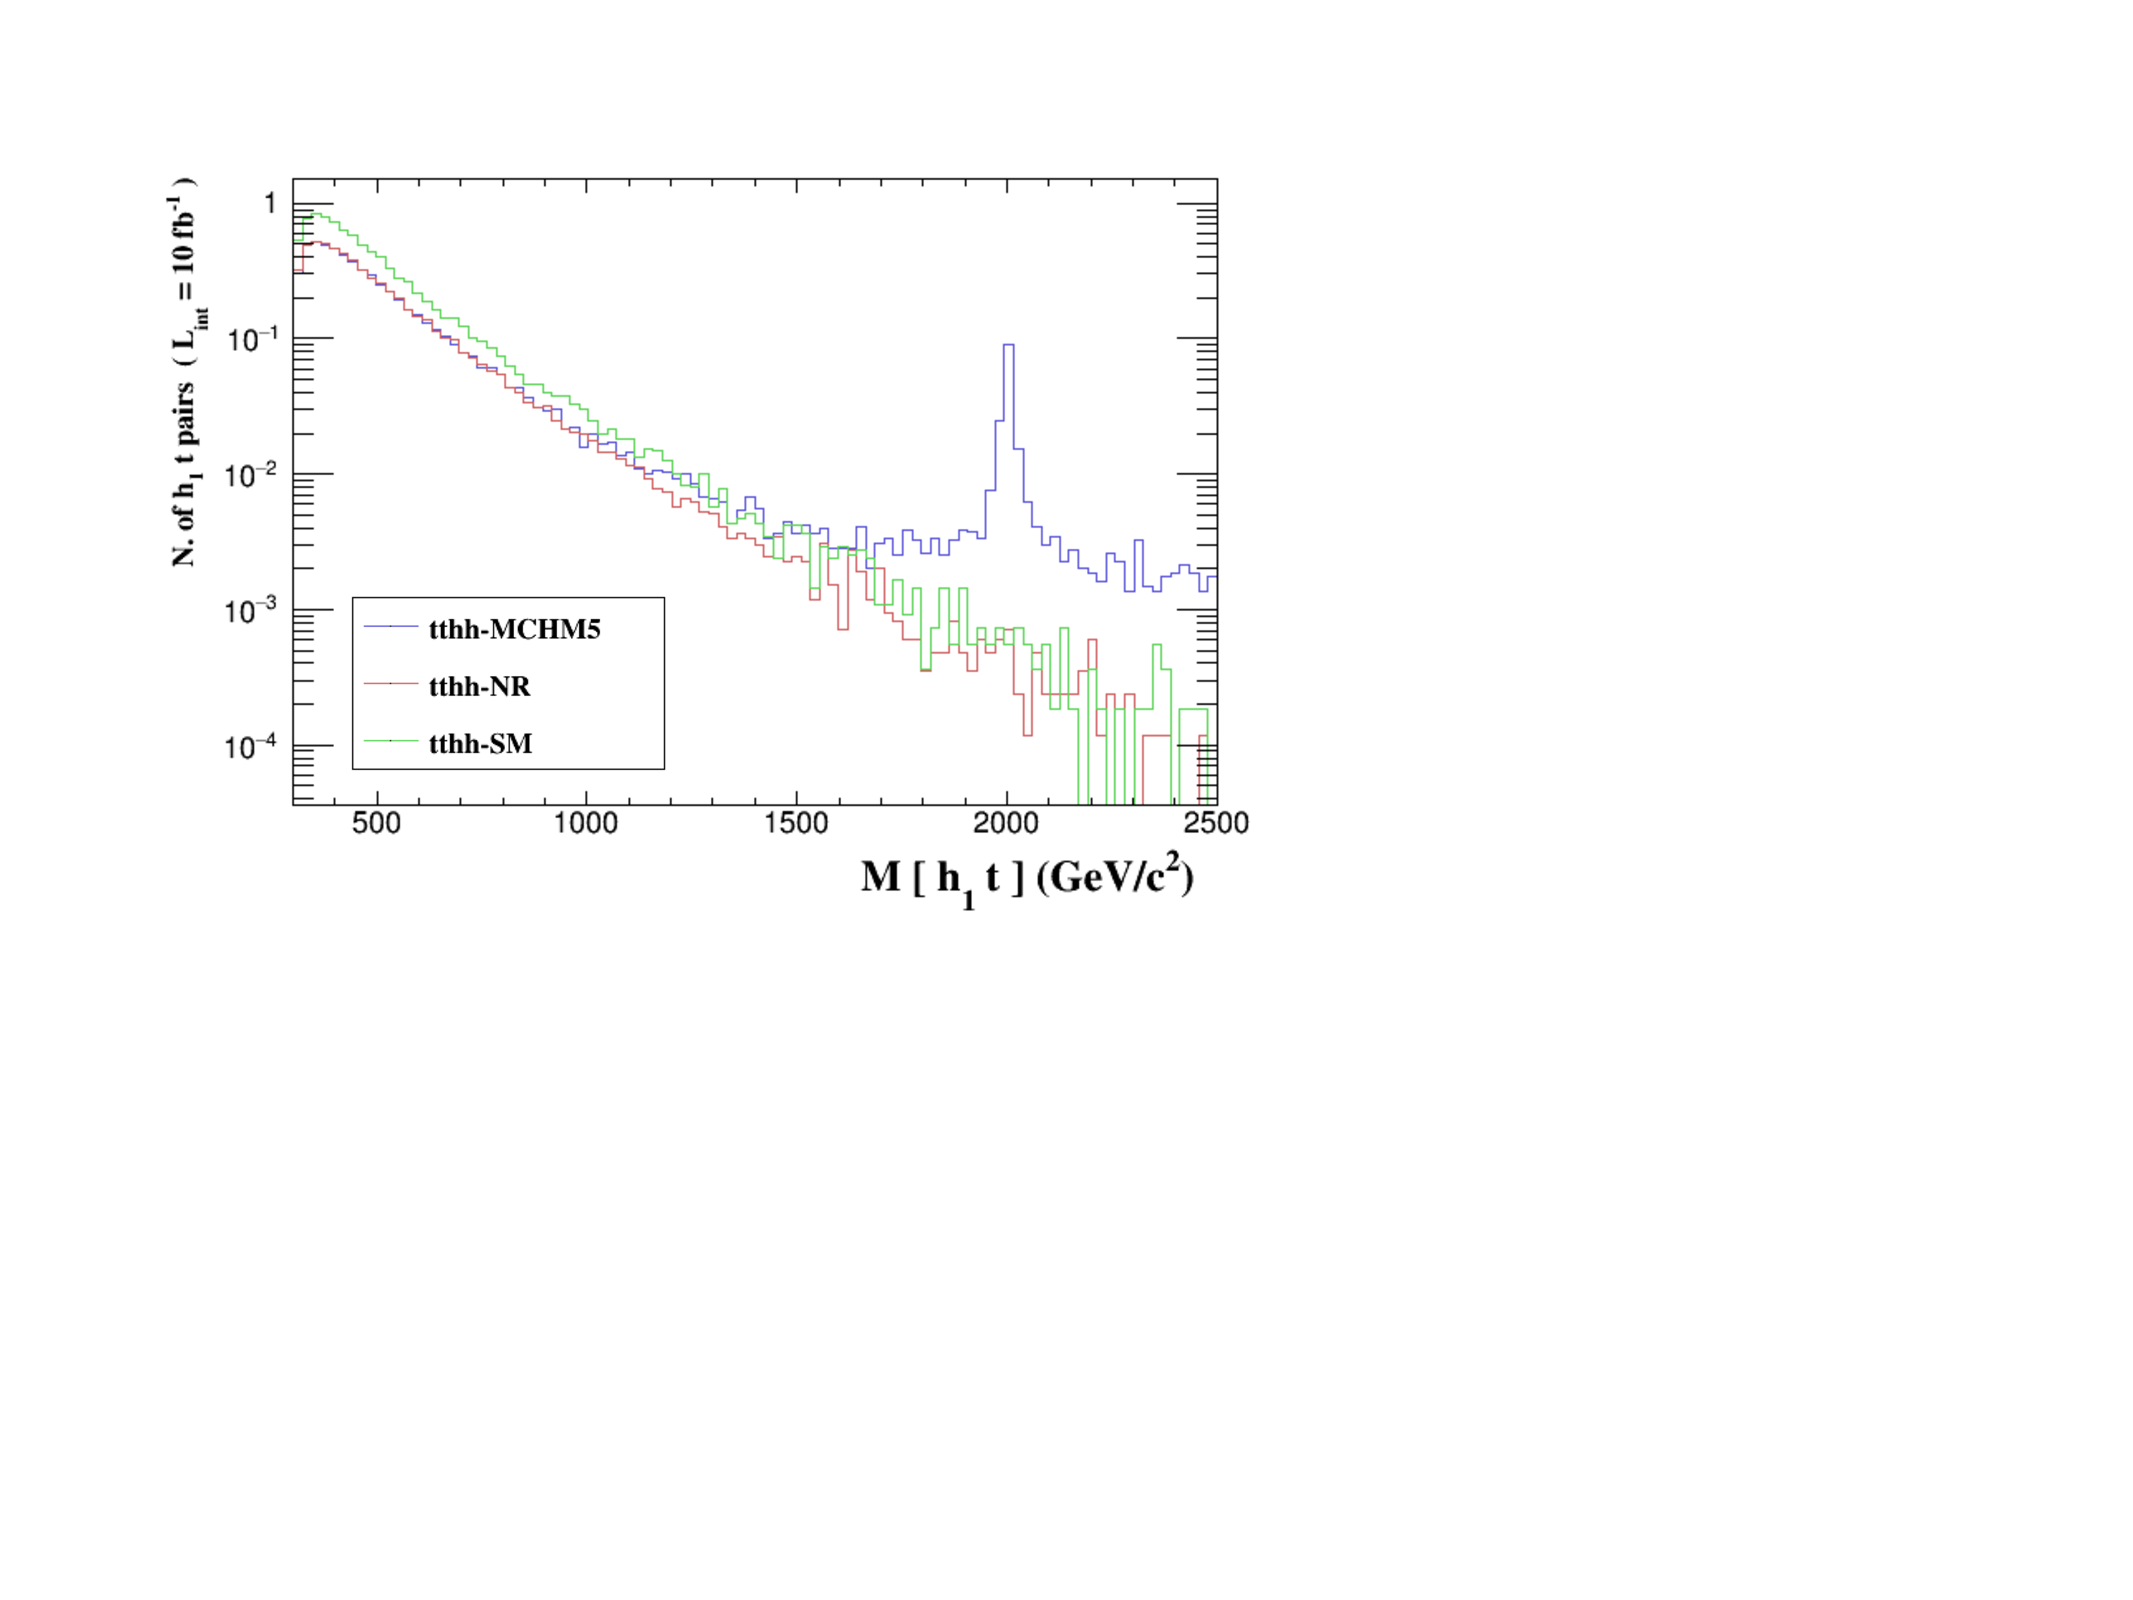
\includegraphics[width=0.48\textwidth]{\main/section9/plots/MCHM5-1-14.pdf}
\put(-110,35){\footnotesize14 \UTeV}
\hspace{3mm}
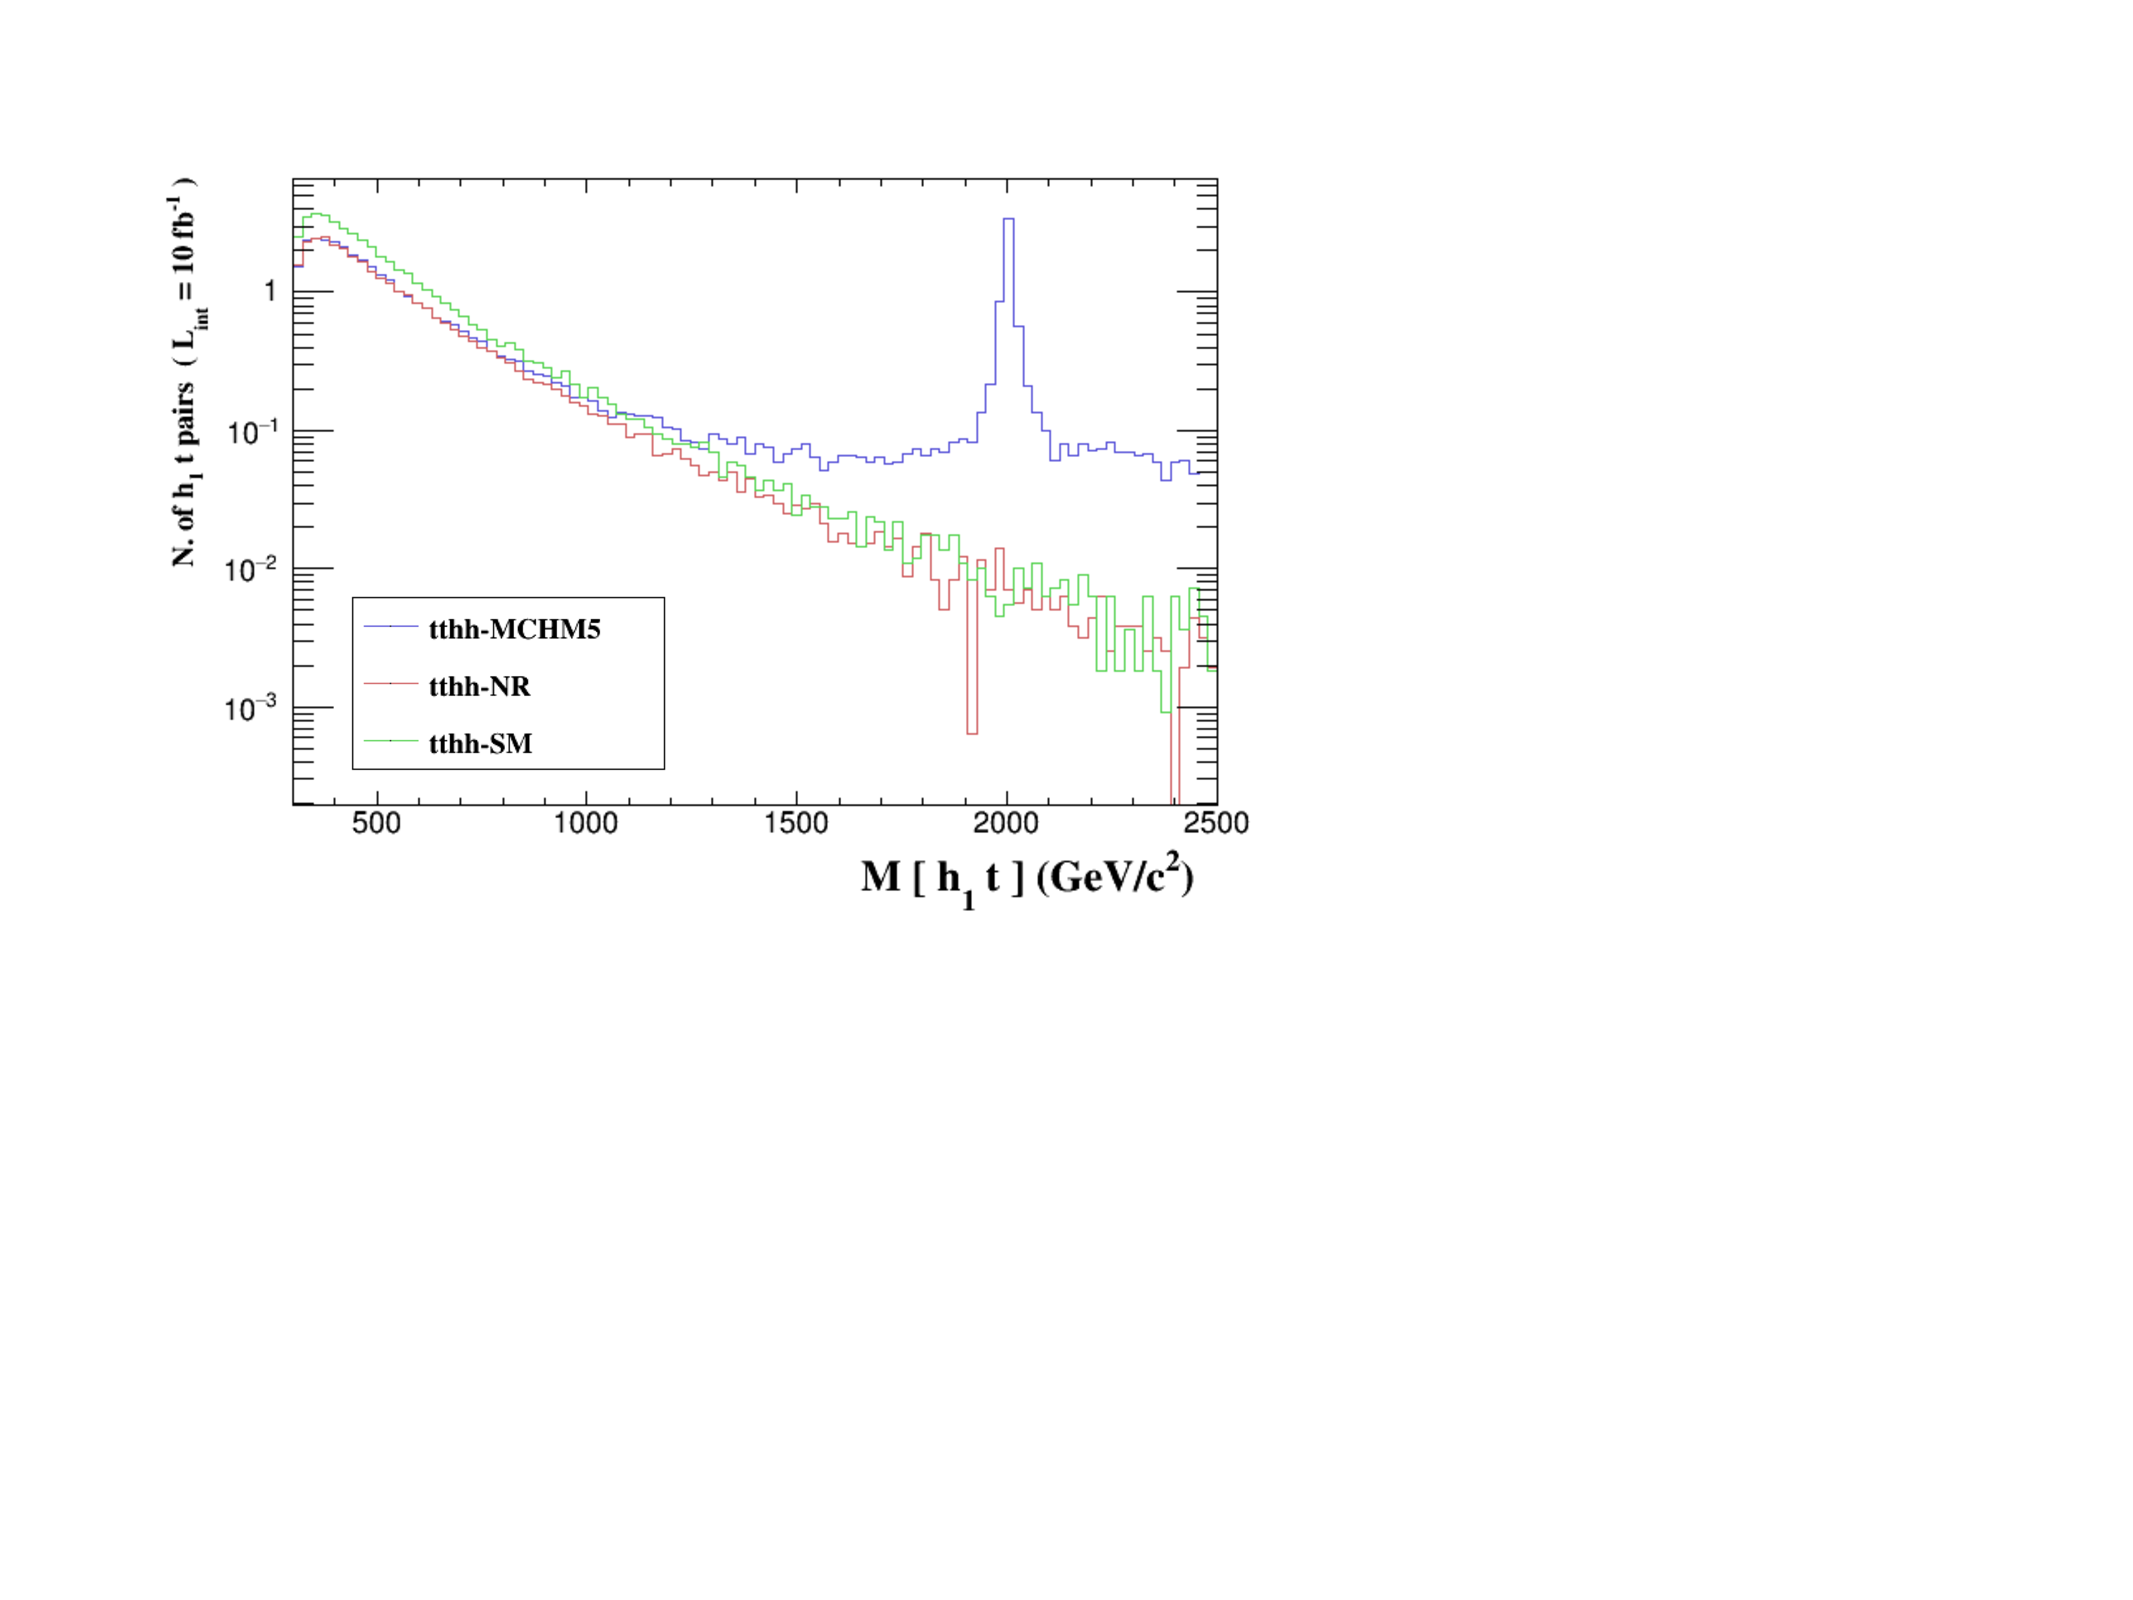
\includegraphics[width=0.48\textwidth]{\main/section9/plots/MCHM5-1-27.pdf}
\put(-110,35){\footnotesize 27 \UTeV} 
\caption{Distribution of the invariant mass of the top quark and the
hardest Higgs boson in the MCHM$_5$ ($M_{1} = -2500$~\UTeV, $M_4 =
2$~\UTeV, $f=1.8$~\UTeV, $y_L=1$).  The blue histogram shows the
distribution of the full $t\bar{t}hh$ process in the MCHM$_5$, while
the NR-$tthh$ cross-section is shown in red.  For comparison, we also
show in green the SM $t\bar{t}hh$ distribution.  Plots generated with
MadAnalysis~5~\cite{Conte:2012fm}.}
\label{fig:htdist}
\end{figure}
%
These contributions may be used to define corresponding ``non-resonant" (NR-$tthh$), and ``resonant" cross sections. The later can lead to important enhancements depending on the masses, while the former carries distinct information. We find that, to an excellent approximation, the total $t\bar{t}hh$ cross-section is given by the sum of these two cross-sections.
%The presence of resonant processes can lead to important enhancements
%in the $t\bar{t}hh$ cross-section w.r.t.~the SM, depending on their
%mass.  The non-resonant process carries information that is distinct
%from the resonant part.  It is therefore useful to
%define a ``non-resonant cross-section" as obtained from this subset of
%diagrams, which we label as ``NR-tthh".  One can similarly define a
%resonant cross section in terms of the diagrams involving QCD
%vector-like pair production.  We find that, to an excellent
%approximation, the total $t\bar{t}hh$ cross-section is given by the
%sum of these two cross-sections. 

In Fig.~\ref{fig:htdist} we show the $ht$ invariant mass distribution
for the resonant and non-resonant processes for a particular point in
the MCHM$_5$.  For comparison, we also show the SM $t\bar{t}hh$
cross-section.  We see that the NR-$tthh$ follows the SM cross-section,
but displays a suppression.  We also see that the relative importance
of the resonant process w.r.t.~the non-resonant one increases with
larger c.m. energies.  The cross-section for both processes also
increases significantly with the c.m. energy (by a factor of 7 in the
total $t\bar{t}hh$ cross-section when going from 14 to 27~\UTeV, and by
a factor of 5 when restricted to NR-$tthh$). 

%%%%%%%%%%%%%%%%%%%%%%%%%%%%%%%%%%%%%%%%%%%%%%%%
\subsubsubsection*{The Non-Resonant $t\bar{t}hh$ Process}
\label{NRtth}
%%%%%%%%%%%%%%%%%%%%%%%%%%%%%%%%%%%%%%%%%%%%%%%%
The diagrams in the MCHM scenarios contributing to the NR-$tthh$ process
fall into three categories:
%
\begin{enumerate}
\item Those that involve only the $ttH$ vertex.
\item Those that involve the trilinear Higgs self-interaction (Section~\ref{sec3}):
$\lambda = \left[ (1 - 2 \xi)/\sqrt{1 - \xi} \right] \lambda_{\rm
SM}$.
\item Those that involve the $ttHH$ vertex (``double Higgs" Yukawa vertex).
\end{enumerate}
%
The first two categories correspond to sets of \textit{diagrams} that
are identical to those in the SM. The third type involves diagrams
that have no counterpart in the SM~\cite{Contino:2012xk}.  The latter
is closely connected to the Higgs compositeness aspect of the MCHM
scenarios, and it would therefore be extremely interesting if one
could get information about such effects experimentally.

By turning off in turn the double Higgs and the trilinear coupling, we find that the effects of the former are
typically at the couple to few percent level in MCHM$_5$ and MCHM$_{14}$ if the $t\bar{t}h$ signal strength,
$\mu(t\bar{t}h) \equiv \sigma(t\bar{t}h)/{\sigma(t\bar{t}h)}_{SM} < 1$, 
and at most $2\%$ in MCHM$_{14}$ if $\mu(t\bar{t}h) > 1$, with a mild dependence
on the c.m. energy (at~14 and 27~\UTeV) in all cases, while the later contributes around $15\%$ in MCHM$_5$ and MCHM$_{14}$ if $\mu(t\bar{t}h) < 1$, and $10\%$ in MCHM$_{14}$ if $\mu(t\bar{t}h) > 1$ at a c.m. energy of 14~\UTeV, decreasing to a few
percent at higher c.m. energies in all cases.  For comparison, the trilinear coupling in the SM $t\bar{t}hh$ cross-section
contributes about $20\%$, with a very mild c.m. energy dependence.  Thus, the NR-$tthh$ is largely determined
by the top Yukawa, being related to the SM process, to a first approximation, by a scaling factor $(y_t / y_t^ {\rm SM})^4$.
This explains the result seen in Fig.~\ref{fig:htdist}, with the
suppression arising from the suppression of the top Yukawa coupling in
the MCHM$_5$.

%In order to get a sense for the relative importance of the different
%physical subprocesses, we simulate the NR-tthh cross section
%turning off, in turn, the double Higgs Yukawa coupling and the trilinear
%coupling.  We find that the effects of the double Higgs Yukawa coupling are
%typically at the couple to few percent level in MCHM$_5$ and MCHM$_{14}$ if the $t\bar{t}h$ signal strength,
%$\mu(t\bar{t}h) \equiv \sigma(t\bar{t}h)/{\sigma(t\bar{t}h)}_{SM} < 1$, 
%and at most $2\%$ in MCHM$_{14}$ if $\mu(t\bar{t}h) > 1$, with a mild dependence
%on the c.m. energy (at~14 and 27~TeV) in all cases.
%We also find that the effect of the trilinear Higgs self-interaction
%can be around $15\%$ in MCHM$_5$ and MCHM$_{14}$ if %$\mu(t\bar{t}h) < 1$, and $10\%$ in MCHM$_{14}$ if %$\mu(t\bar{t}h) > 1$ at a c.m. energy of 14~TeV, decreasing to a %few
%percent at higher c.m. energies in all cases.  For comparison, %the effect of the
%trilinear Higgs self-interaction in the SM $t\bar{t}hh$ cross-section
%is about $20\%$, with a very mild c.m. energy dependence.  Thus, the
%NR-tthh (like the SM $t\bar{t}hh$ cross-section) is largely determined
%by the top Yukawa interaction, and the two are, to a first
%approximation, related by a scaling factor $(y_t / y_t^ {\rm SM})^4$.
%This explains the result seen in Fig.~\ref{fig:htdist}, with the
%suppression arising from the suppression of the top Yukawa coupling in the MCHM$_5$.


The previous observation also leads to a strong correlation between the $t\bar{t}h$ and the NR-$tthh$ processes, as shown in Fig.~\ref{fig:nrtthhvstth}. Due to the different scaling with the top Yukawa coupling, the deviations from the SM in the NR-$tthh$ process are larger than those in $t\bar{t}h$.
%%%%%%%%%%%%%%%%%%%%%%%%%%%%%%%%%%%%%%%%%%%%%%%%
%\subsubsubsection{Sample Points}%
\subsubsubsection*{Set of Example Points}
\label{benchmarks}
%%%%%%%%%%%%%%%%%%%%%%%%%%%%%%%%%%%%%%%%%%%%%%%%
We show in Table \ref{fig:benchmarkTable1} 
%and \ref{fig:benchmarkTable2}, 
a number of points selected as examples that illustrate, in
more detail, the properties of the MCHM$_5$ and MCHM$_{14}$.  
%They are indicated in% 
These properties are reflected in Figs.~\ref{fig:nrtthhvstth}, ~\ref{fig:tthvsf} and~\ref{fig:tthhvsMT4}, where these points are indicated. The MCHM$_5$ points are labelled as P$_i$, i=1 to 5, and MCHM$_{14}$ points as P'$_j$, with j=1 to 4.
%
\begin{table}[t]
\centering
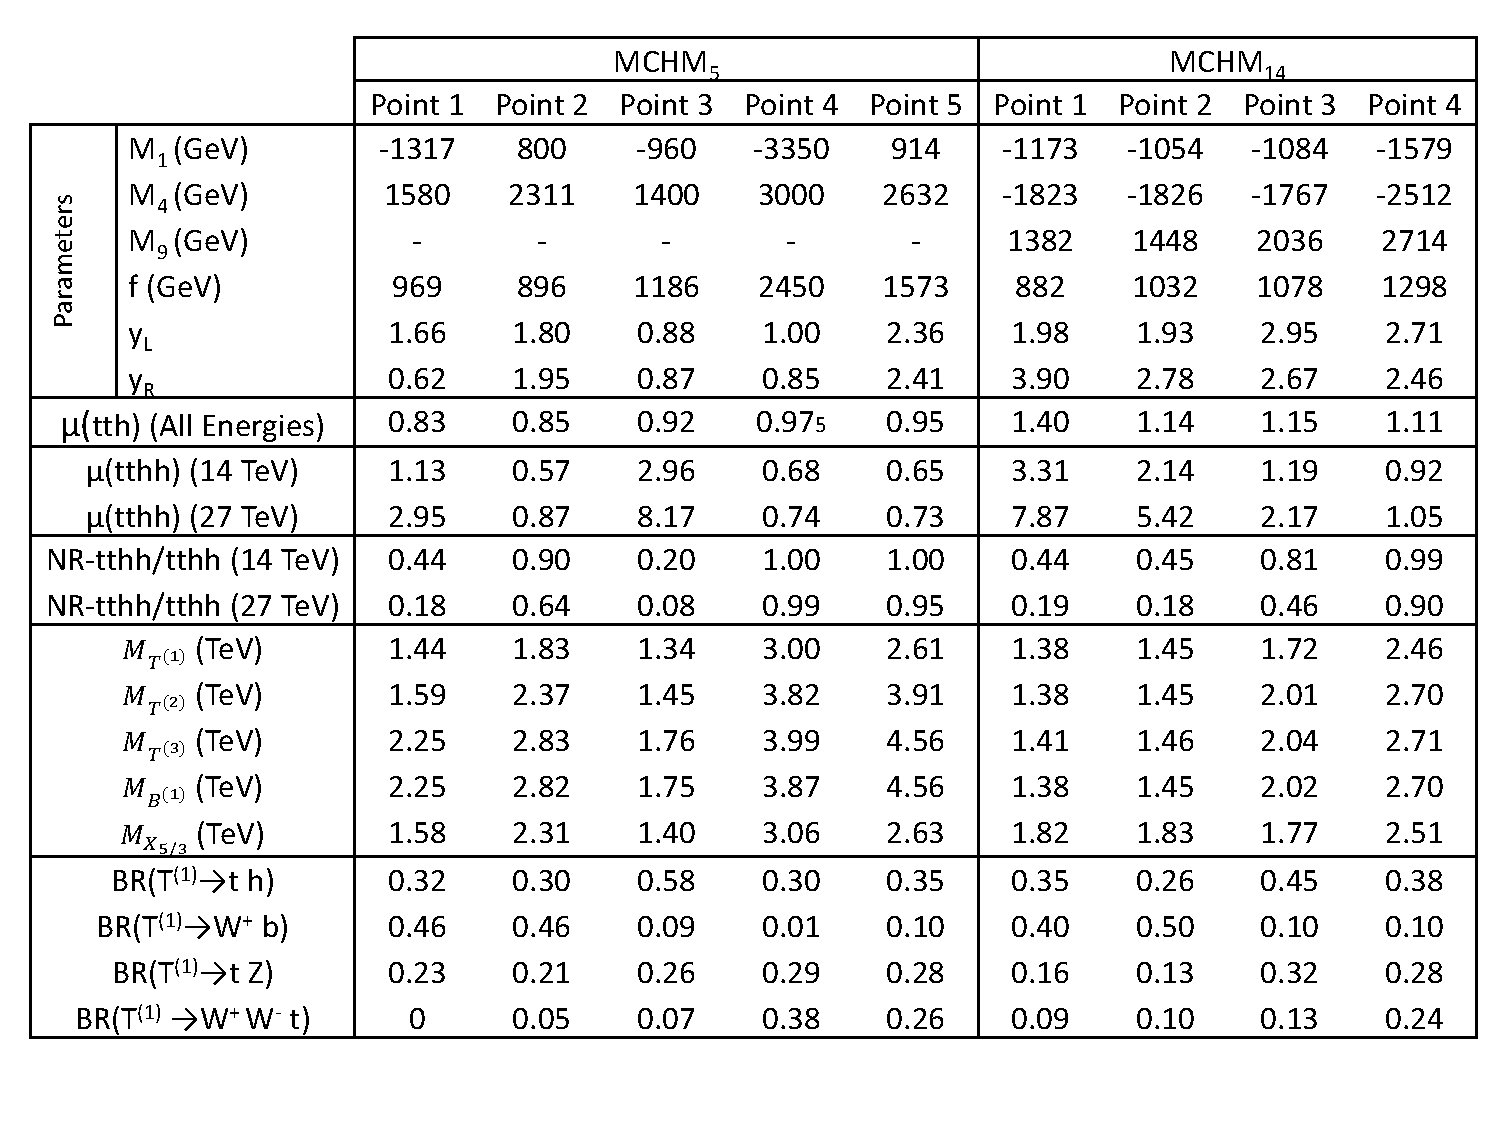
\includegraphics[width=0.85\textwidth]{\main/section9/plots/ExamplePoints_MCHM5_14.pdf}
\caption{Sample points for MCHM$_5$ with M$_1$ M$_4$ same sign and opposite sign and for MCHM$_{14}$ with M$_1$ and M$_4$ both $<0$ and $\mu({\rm ttH})>1$.}
\label{fig:benchmarkTable1}
\end{table}
%
\begin{figure}[t]
\centering
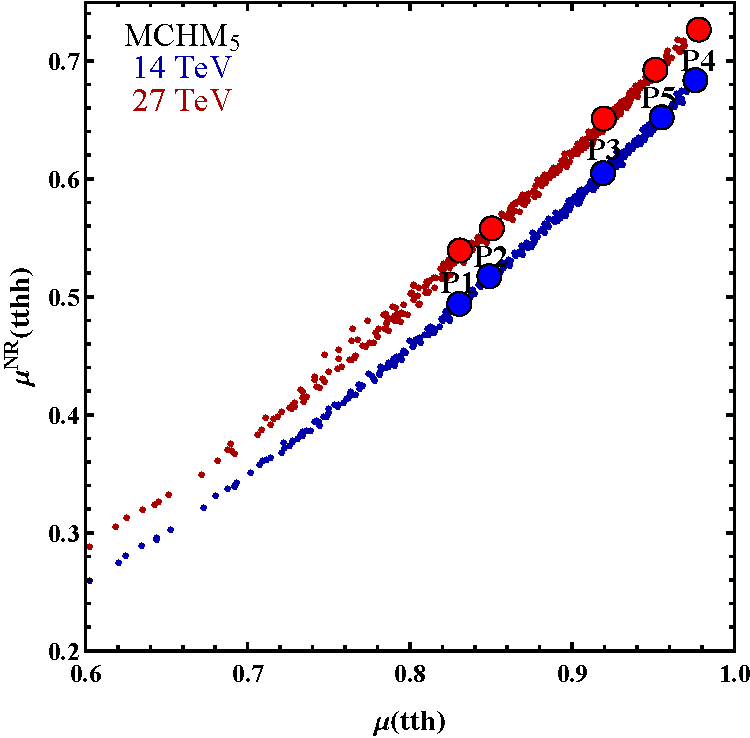
\includegraphics[width=0.4\textwidth]{\main/section9/plots/MCHM5_XStth_Norm_XStthh_NR_Norm-14_and_27.pdf}
\hspace{1.5cm}
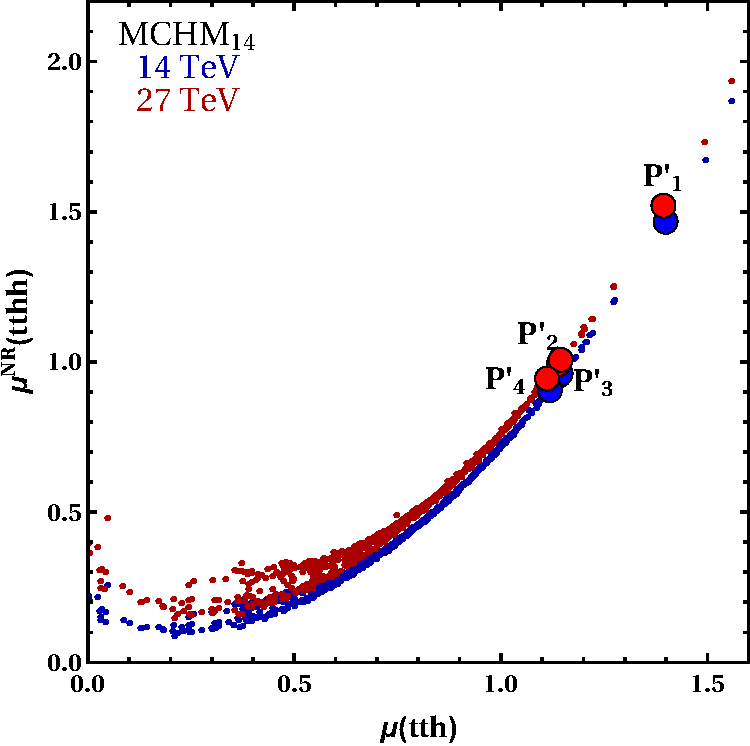
\includegraphics[width=0.4\textwidth]{\main/section9/plots/MCHM14_XStth_Norm_XStthh_NR_Norm-14_and_27.pdf}
\caption{Correlation between the $t\bar{t}h$ and
non-resonant $t\bar{t}hh$ signal strengths ($\mu$), for 14 and 27~\UTeV c.m.~energies. The left (right) plots correspond to the MCHM$_5$ (MCHM$_{14}$)}
\label{fig:nrtthhvstth}
\end{figure}
%
The points for the MCHM$_5$ exhibit a suppression in $\mu(t\bar{t}h)$ that ranges from about 15\% (roughly at the current
95\% C.L.~limit~\cite{Aaboud:2018urx, Sirunyan:2018hoz}) to a few
percent, a sensitivity that might be achievable by the end of the HL
phase of the LHC run, with smaller deviations from the SM for larger values of $f$ (Fig~\ref{fig:tthvsf},a). The Table ~\ref{fig:benchmarkTable1} and Fig~\ref{fig:tthhvsMT4} show that the
$t\bar{t}hh$ process can exhibit an enhancement for light enough
resonances, increasing with higher c.m.~energy, as expected. For points 2, 4 and 5 in the MCHM$_{5}$, the resonant production is not enough to produce an
enhancement in $t\bar{t}hh$ compared to the SM, although these points correspond to two different cases; the resonances for Point 2 are slightly beyond the current direct limit whereas, on the contrary, much beyond that limit for points 4 and 5. In this case, the
$t\bar{t}hh$ process is easily dominated by the NR-$tthh$ process, as
defined above.  
%The points for the MCHM$_5$ exhibit a suppression in $\mu(t\bar{t}h)$ that ranges from about 15\% (roughly at the current
%95\% C.L.~limit~\cite{Aaboud:2018urx, Sirunyan:2018hoz}) to a few
%percent, a sensitivity that might be achievable by the end of the HL
%phase of the LHC run (Fig.~\ref{fig:tthvsf},a).  The smaller deviations from the SM are
%associated with larger values of $f$ (Fig~\ref{fig:tthvsf},a).  The Table 19 and Fig~\ref{fig:tthhvsMT4} show that the
%$t\bar{t}hh$ process can exhibit an enhancement if the fermion
%resonances are light enough.  As expected, this enhancement increases
%with increasing c.m.~energy. For the points 2, 4 and 5 in the MCHM$_{5}$, the resonant production is not enough to produce an
%enhancement in $t\bar{t}hh$ compared to the SM, although these points correspond to two different cases; the resonances for Point 2 are slightly beyond the current direct limit whereas, on the contrary, much beyond that limit for points 4 and 5. In this case, the
%$t\bar{t}hh$ process is easily dominated by the NR-tthh process, as
%defined above.  For completeness, Table~\ref{fig:benchmarkTable1} includes the
%spectrum of resonances, and the BRs for the lightest $Q=2/3$ one.  It
%decays mostly into the standard $th$, $Wb$ and $tZ$ channels (with BRs
%that are model dependent), but in some cases it has a non-negligible
%non-standard BRs, such as into the $W^+W^- t$ channel.

The set of example points for MCHM$_{14}$ in Table~\ref{fig:benchmarkTable1} exhibits an enhancement of the top Yukawa
coupling, due to the effect described above and reflected in Fig~\ref{fig:tthvsf},b.  These
enhancements can easily be of the order of 10-20\%.  Interestingly,
Point 1 shows that the enhancement can be as large as 40\% (while
being consistent with a sufficiently small deviation in the $ggh$
vertex~\cite{MCHMtthh}). The four points display as well, an enhancement
in the $t\bar{t}hh$ process.  While about half of the rate is due to
resonant production in Points 1 and 2, for points 3 and 4 the
enhancement arises dominantly from the non-resonant process,
reflecting the enhancement in the top Yukawa coupling. All the selected points for MCHM$_{14}$ lie in the
$M_1 < 0$, $M_4 < 0$ quadrant of the right panel of
Fig.~\ref{fig:ytvsM1M4}. The properties of the other quadrants are
qualitatively rather similar to those of the MCHM$_5$ (see~\cite{MCHMtthh}).

For completeness, Table~\ref{fig:benchmarkTable1} includes the
spectrum of the 5 resonances in the MCHM$_{5}$, and of the 3 lightest 2/3 resonances, the lightest B resonance and the lightest 5/3 resonance out of the total of 14 resonances of the MCHM$_{14}$, as well as the BRs for the lightest $Q=2/3$ one.  It
decays mostly into the standard $th$, $Wb$ and $tZ$ channels (with BRs
that are model dependent), but in some cases it has non-negligible
non-standard BRs, such as into the $W^+W^- t$ channel.  
%The set of example points for MCHM$_{14}$ in Table~\ref{fig:benchmarkTable1} exhibits an enhancement of the top Yukawa
%coupling, due to the effect described in Section~\ref{MCHM} and reflected in Fig~\ref{fig:tthvsf},b.  These
%enhancements can easily be of the order of 10-20\%.  Interestingly,
%Point 1 shows that the enhancement can be as large as 40\% (while
%being consistent with a sufficiently small deviation in the $ggh$
%vertex~\cite{MCHMtthh}).  The four points display as well, an enhancement
%in the $t\bar{t}hh$ process.  While about half of the rate is due to
%resonant production in Points 1 and 2, for points 3 and 4 the
%enhancement arises dominantly from the non-resonant process,
%reflecting the enhancement in the top Yukawa coupling.  In Table~\ref{fig:benchmarkTable1} are displayed,
% the spectrum of the 5 resonances in the MCHM$_{5}$ and of the 3 lightest 2/3 resonances, the lightest B resonance and the lighest 5/3 resonance out of the total of 14 resonances of the MCHM$_{14}$.  
% All the selected points for MCHM$_{14}$ lie in the
%$M_1 < 0$, $M_4 < 0$ quadrant of the right panel of
%Fig.~\ref{fig:ytvsM1M4}. The properties of the other quadrants are
%qualitatively rather similar to those of the MCHM$_5$ (see~\cite{MCHMtthh}).
\begin{figure}[!htb]
\centering
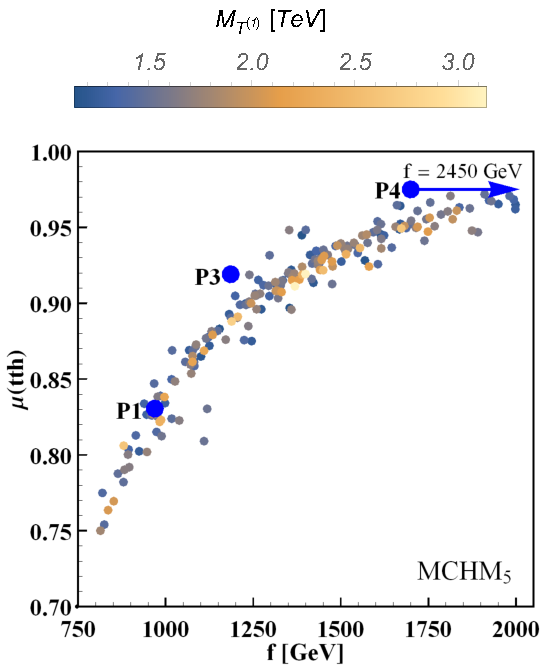
\includegraphics[width=0.4\textwidth]{\main/section9/plots/MCHM5_f_XStth_Norm_MT4_Q2.pdf}
\put(-35,45){a)}
\hspace{1.5cm}
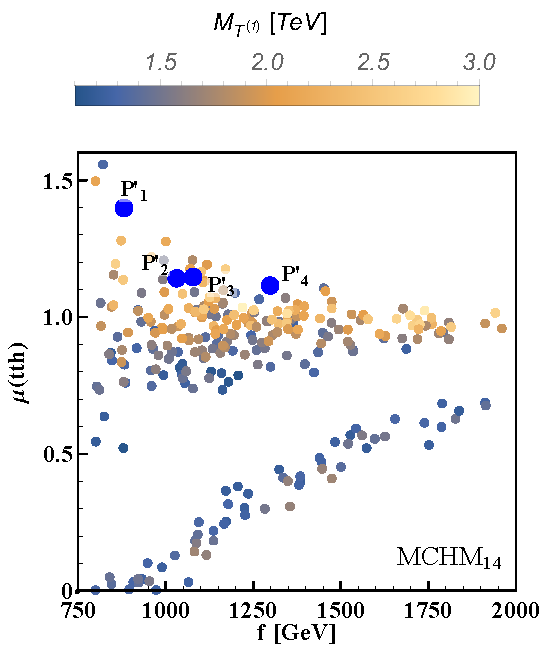
\includegraphics[width=0.417\textwidth,scale=1.2]{\main/section9/plots/MCHM14_f_XStth_Norm_MT4_Q3.pdf}
\put(-45,45){b)}
\caption{The $t\bar{t}h$ signal  strength as a function of the $f$-scale,
for 14 and 27~\UTeV c.m. energies, with colour coded the lightest
vector-like mass.  The left (right) plots correspond to Q2 of MCHM$_5$ (Q3 of MCHM$_{14}$). The blue arrow indicates that the point P4 is outside the horizontal range of the plot with f=2450 \UGeV.}
\label{fig:tthvsf}
\end{figure}
\begin{figure}[!htb]
\centering
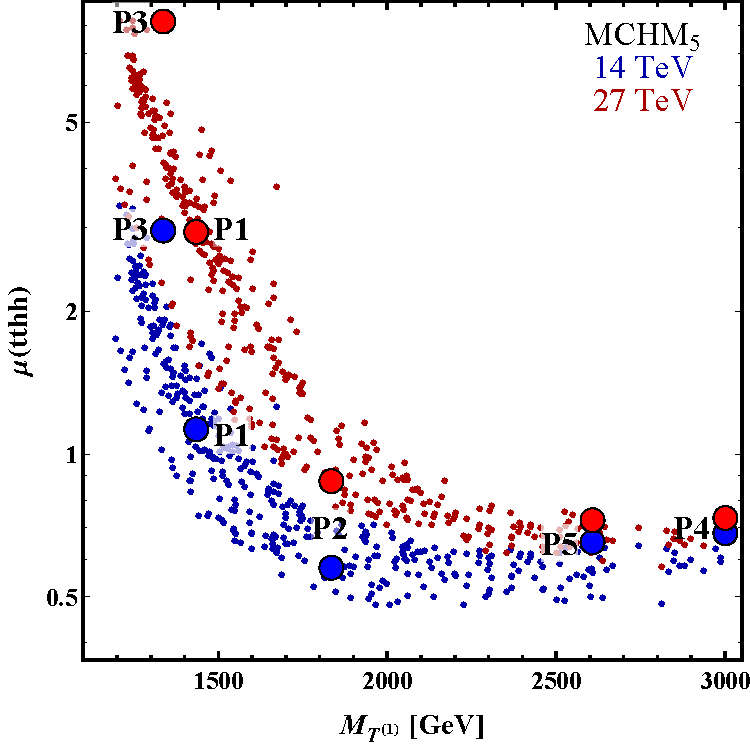
\includegraphics[width=0.4\textwidth]{\main/section9/plots/MCHM5_MT4_XStthh_Norm-14_and_27.pdf}
\put(-60,171){a)}
\hspace{1.5cm}
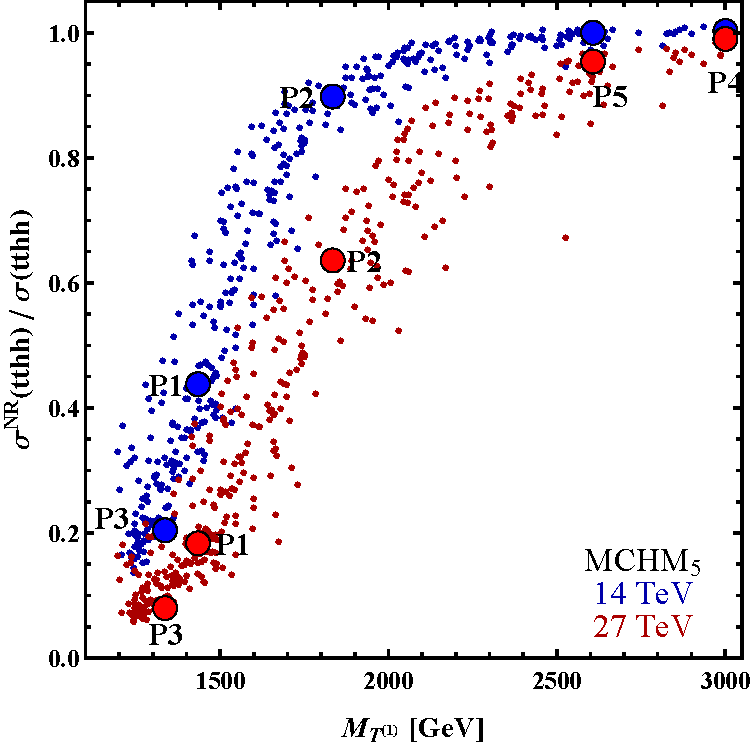
\includegraphics[width=0.4\textwidth]{\main/section9/plots/MCHM5_MT4_XStthh_NR_over_XStthh-14_and_27.pdf}
\put(-60,45){b)}
\caption{The left plot shows the $t\bar{t}hh$ signal  strength as a function of the
lightest $Q = 2/3$ vector-like mass, T$^{(1)}$ for 14 and 27~\UTeV c.m. energies for the MCHM$_5$. The right plot shows the ratio between the non-resonant $t\bar{t}hh$ cross section and the total $t\bar{t}hh$ cross section as a function of T$^{(1)}$
% the lightest $Q = 2/3$ vector-like mass,%
for 14 and 27~\UTeV c.m. energies for the MCHM$_5$.}
\label{fig:tthhvsMT4}
\end{figure}
%
%%%%%%%%%%%%%%%%%%%%%%%%%%%%%%%%%%%%%%%%%%%%%%%%
\subsubsection*{Experimental perspectives}
\label{perpectives}
%%%%%%%%%%%%%%%%%%%%%%%%%%%%%%%%%%%%%%%%%%%%%%%%
%
A deviation from the SM in the $t{\bar t}h$ production is an essential measurement for MCHM. An increase will reject the MCHM$_5$ scenario and greatly refine the areas of the parameter space where MCHM$_{14}$ would be valid. A deficit instead, would make MCHM$_5$ and MCHM$_{14}$ both possible. The measurement of this observable is expected to be achieved within 5\% accuracy at the HL-LHC (Sections~\ref{sec2:top},\ref{sec2:exp_combination},\ref{sec2:exp_kappa}) and thus with very high accuracy at HE-LHC. The $t{\bar t}hh$ production process plays a major role in MCHM searches. Deviations from the SM expectation (deficit or increase) can be significant in both MCHM scenarios. The $t{\bar t}hh$ production cross-section is around 1 fb (Section~\ref{sec:HH_NLO}) at tree level whereas $t{\bar t}h$ is about 500 times larger (Section~\ref{sec2_HXSWG1}). Therefore the aim at HL-LHC will be to evidence this process and discover if a strong deviation from SM. Higher energy together with higher luminosity (HE-LHC) will further explore MCHM.


\textbf{Acknowledgements:}
This work was supported by the S\~ao Paulo Research Foundation
(FAPESP) under Grants No.~2016/01343-7, No.~2013/01907-0,
No.~2015/26624-6 and No.~2018/11505-0 and by Science Without Borders/CAPES for UNESP-SPRACE under the Grant No.~88887.116917/2016-00.
